\section{Metodologia}

\subsection{Sistema massa–mola}

Utilizou-se um conjunto composto por suporte metálico, molas de diferentes constantes elásticas e três massas calibradas, sendo duas delas de 100 gramas e uma de 200 gramas. Cada massa foi acoplada à extremidade inferior da mola, a qual foi fixada ao suporte. A massa foi então deslocada verticalmente e solta, iniciando oscilações. O experimento foi repetido com diferentes massas e molas e foi registrado no formato de vídeo para análises posteriores utilizado o software \textit{Tracker}.

A \cref{fig:massamola} apresenta o sistema massa–mola montado e os componetes utilizados.

\begin{figure}[H]
    \centering
    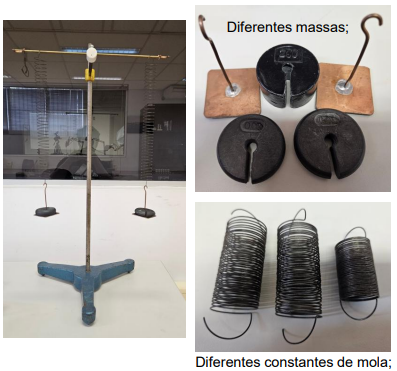
\includegraphics[width=0.35\linewidth]{fig/massamola.png}
    \caption{A esquerda, o sistema massa–mola com as massas acopladas à extremidade inferior da mola, a direita, jogo de molas, pesos e suportes utilizados no experimento. Fonte: Fotografias tiradas pelo monitor Pedro}
    \label{fig:massamola}
\end{figure}

\subsection{Pêndulo de Wilberforce}

O pêndulo de Wilberforce foi composto por uma mola helicoidal disposta verticalmente, acoplada em sua extremidade inferior a um cilindro metálico. Este cilindro continha discos de dimensões semelhantes, conectados por meio de uma haste metálica, com posições ajustáveis ao longo do eixo, permitindo o controle da distribuição de massa. Essa configuração possibilita ao sistema oscilar simultaneamente nos modos vertical e rotacional. A extremidade superior da mola foi fixada a um suporte rígido, sustentando o conjunto oscilante.. O sistema foi iniciado com oscilação exclusivamente vertical, observando-se posteriormente o acoplamento com o movimento rotacional.

A \cref{fig:wilberforce} mostra o sistema em repouso e a representação gráfica do seu movimento.

\begin{figure}[H]
    \centering
    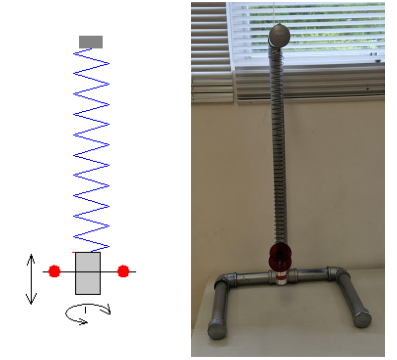
\includegraphics[width=0.35\linewidth]{fig/wilberforce.png}
    \caption{Pêndulo de Wilberforce à direita e representação do moviemnto do cilindro oscilando vertical e angularmente à esquerda. Fonte: Fotografia tirada pelo monitor Pedro e imagem disponibilizada pelo mesmo.}
    \label{fig:wilberforce}
\end{figure}

\subsection{Pêndulo de torção}

Utilizou-se um fio metálico fino, fixado na extremidade superior, com um cilindro metálico contendo uma fita métrica em seu entorno suspenso em sua extremidade inferior. O sistema realizou oscilações angulares em torno do eixo do fio. O tempo para 10 oscilações foi registrado com cronômetro digital. O experimento foi realizado em dois meios: ar e óleo. No segundo caso, o cilindro foi parcialmente imerso. Foram utilizados os cinco primeiros valores de tempo de cada meio para plotar um gráfico e realizar sua linearização por meio da ferramenta do Google Planilhas, com o objetivo de prever o valor correspondente a dez oscilações e, posteriormente, compará-lo com os dados obtidos empiricamente.

A \cref{fig:torsao} mostra o pêndulo de torção e os componentes utilizados no experimento.

\begin{figure}[H]
    \centering
    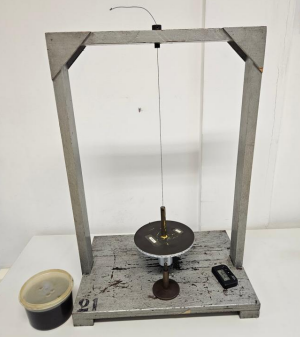
\includegraphics[width=0.35\linewidth]{fig/torsao.png}
    \caption{Materiais utilizados: pêndulo de torção, recipiente contendo óleo e cronômetro. Fonte: Fotografia tirada pelo monitor Pedro}
    \label{fig:torsao}
\end{figure}

\subsection{Propagação de ondas em molas}

Foram utilizadas duas molas com diferentes rigidezes, dispostas horizontalmente sobre superfície plana. Ondas transversais e longitudinais foram geradas por impulsos aplicados manualmente em uma extremidade da mola tensionada. Observou-se a propagação da perturbação, a formação de nós e padrões de interferência.

A \cref{fig:ondas} mostra as difrentes molas utilizadas para a realização desse experimento.

\begin{figure}[H]
    \centering
    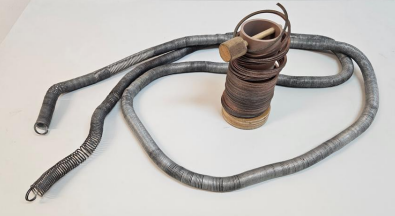
\includegraphics[width=0.35\linewidth]{fig/ondas.png}
    \caption{Sistema de molas utilizadas no experimento. Fonte: Fotografia tirada pelo monitor Pedro}
    \label{fig:ondas}
\end{figure}

\subsection{Esfera vibrando}

Uma esfera de plástico acoplada a um excitador eletromecânico em seu interior foi suspensa por uma corda. O dispositivo foi ligado gerando perdubações na corda suspensa, o comprimento da corda foi ajustado até que padrões de ondas estacionárias fossem observados na mesma. 

A \cref{fig:esfera} ilustra a esfera utilizada no experimento e a corda em que os padrões descritos foram observados.

\begin{figure}[H]
    \centering
    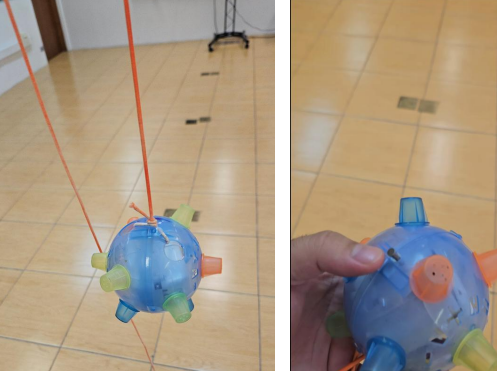
\includegraphics[width=0.35\linewidth]{fig/esfera.png}
    \caption{Esfera plástica com o excitador interno desligado suspensa por um corda e repolsanda sobre uma mão. Fonte: Fotografias tiradas pelo monitor Pedro}
    \label{fig:esfera}
\end{figure}
